\section{Homotopies}  

\subsection{Homotopy and Path Homotopy}

  The concept of homotopies is dealt with in algebraic topology, but it is worthwhile to mention it now. 

  \begin{definition}[Homotopy]
    Two continuous paths from $x$ to $y$ in topological space $X$ is \textbf{homotopic} if one can be continuously "deformed" into the other, such a deformation being the \textbf{homotopy} between two functions. The set of linearly homotopic paths form a relation, and thus \textbf{homotopy classes} can be further defined. 
    \begin{figure}[H]
      \centering 
      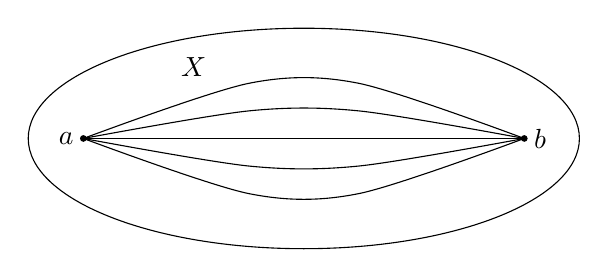
\begin{tikzpicture}[scale=0.7]
        \draw (0,0) ellipse (5 and 2);
        \draw[fill] (-4,0) circle (0.05);
        \draw[fill] (4,0) circle (0.05);
        \draw plot [smooth] coordinates {(-4,0) (-1,1) (1,1) (4,0)};
        \draw (-4,0)--(4,0);
        \draw plot [smooth] coordinates {(-4,0) (-1,0.5) (1,0.5) (4,0)};
        \draw plot [smooth] coordinates {(-4,0) (-1,-0.5) (1,-0.5) (4,0)};
        \draw plot [smooth] coordinates {(-4,0) (-1,-1) (1,-1) (4,0)};
        \node at (-2,1.3) {$X$};
        \node[left] at (-4,0) {$a$};
        \node[right] at (4,0) {$b$};
      \end{tikzpicture}
      \caption{Visually, the set of all the curves in the space $X$ as shown are in a single homotopy class.} 
      \label{fig:single_homotopy_class}
    \end{figure}
  \end{definition}

  It is clear that the space $X$ consists of a single homotopy class of curves from $a$ to $b$. However, a space may have an infinite number of such classes. 

  \begin{figure}[H]
    \centering 
    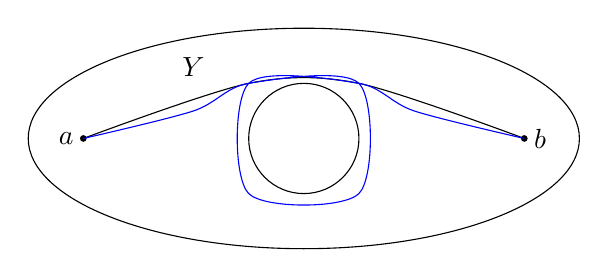
\begin{tikzpicture}[scale=0.7]
      \draw (0,0) ellipse (5 and 2);
      \draw[fill] (-4,0) circle (0.05);
      \draw[fill] (4,0) circle (0.05);
      \draw plot [smooth] coordinates {(-4,0) (-1,1) (1,1) (4,0)};
      \node[left] at (-4,0) {$a$};
      \node[right] at (4,0) {$b$};
      \draw (0,0) circle (1);
      \node at (-2,1.3) {$Y$};
      \draw[blue] plot [smooth] coordinates {(-4,0) (-2,0.5) (-1,1) (1,1) (1,-1) (-1,-1) (-1,1) (1,1) (2,0.5) (4,0)};
    \end{tikzpicture}
    \caption{Let us define the space $Y \equiv X \setminus C$ where $C$ is a circular region in $X$. Then, $Y$ has an infinite number of homotopy classes. We show two curves, that are in two different homotopy classes. }
    \label{fig:homotopy_class}
  \end{figure}

  \begin{definition}[Simply Connected Set]
    A \textbf{simply connected set} is a set such that all paths between any two given points are homotopic. That is, a simply connected set has one homotopy class. 
  \end{definition}

\subsection{The Fundamental Group}

